\documentclass[ukrainian,utf8,simple,floatsubsection, hpadding=5mm,equationsubsection,]{eskdtext}
\usepackage[warn]{mathtext}
\usepackage[unicode]{hyperref} % enable hyperlinks (активувати посилання)
\usepackage{amssymb} % special math characters
\usepackage{amsmath} % using cyrillic in formulae
\usepackage{amsfonts} % special math fonts
\usepackage{eskdtotal} 
\usepackage{graphicx,epstopdf} % epstopdf-convert eps files to pdf
\graphicspath{{algorithms/}{schemes/}{software/}{fig/}} % look up folders for figures
\usepackage{listings} % to add source codes
\usepackage{longtable} % multipage tables
\usepackage{multirow} % using rowspan in tables
\usepackage{nomencl} % support for abbreviations
\makenomenclature % generate abbrevs index file
\usepackage{float}
% variables.tex
% This file contains information about author and other specific
% people for use in eskdx collection.

\title{\fontsize{12}{12} \selectfont Інтегрована інерціально-супутникова система навігації, що базується на принципах комплексної обробки інформації
з використанням калманівської фільтрації}
% smaller size of font set for the title in frame
\author{НовікМ.В.}

\ESKDchecker{ФіляшкінМ.К.}
\ESKDnormContr{КозловА.П.}
\ESKDapprovedBy{СинєглазовВ.М.}

\ESKDdepartment{Міністерство освіти і науки України}
\ESKDcompany{Національний авіаційний університет}

\ESKDsignature{НАУ 11 09 02 000 ПЗ}
\ESKDgroup{ІАСУ 608}

\ESKDsectAlign{section}{Center}
\ESKDsectAlign{subsection}{Center}
\ESKDsectAlign{subsubsection}{Center}

 % class parameters tuning
\ESKDcolumnXIfIV{РусаловськийА.В.}
\ESKDstyle{formIIab}
\renewcommand\labelenumi{\arabic{enumi}.} 
\renewcommand\labelenumii{\theenumi.\arabic{enumii}.}
\renewcommand\labelenumiii{\arabic{enumi}.\arabic{enumii}.\arabic{enumiii}.}
\begin{document}
\ESKDthisStyle{formII}




\section{Охорона праці}
\subsection{Вступ}

В дипломній роботі розробляється інерціально-супутникова навігаційна система, що базується на основі комплексної обробки інформації з використанням фільтра Калмана. Розробкою та відпрацюванням алгоритмів роботи навігаційної системи, налаштуванням обладнання та калібровкою датчиків займаються інженери програмісти та радіотехніки лабораторії. Отже суб’єктом є інженер програміст лабораторії, функціональним зобов'язаннями якого є програмування навігаційних алгоритмів для бортової обчислюваної машині, засобом праці є персональний комп'ютер та модулі навігаційного обладнання: датчики навігаційної системи (мікромеханічні чи лазерні акселерометри та гіроскопи), бортовий обчислювач навігаційної інформації.

До роботи з навігаційним обладнанням та ЕОМ допускаються працівники, що не мають медичних протипоказань, пройшли вчасно періодичний медичний огляд, інструктаж і навчання  правилам техніки безпеки і виробничої санітарії.

Основним місцем роботи інженера програміста є лабораторія навігаційного обладнання авіаційного підприємства чи науково-дослідного інституту. Періодично місцем роботи може бути літак, де встановлено навігаційне обладнання (налаштування, тестування, випробування) або ЗПС, у випадку, якщо розробляємі пристрої встановлюються на БПЛА.

\subsection{Опис робочого місця}
Для приміщення лабораторії вибрана площа 30 $\text{м}^2$, з висотою стелі -- 3м. Виробничі будівлі та приміщення споруджуються згідно з вимогами будівельних і санітарних норм. Об’єм виробничих приміщень для програмістів, операторів відеотермінальних пристроїв на одного працівника складає 19,5 $\text{м}^2$, площа приміщень — 6 м2 з урахуванням максимального числа працівників в одну зміну. 

\begin{figure}[H]
\centering
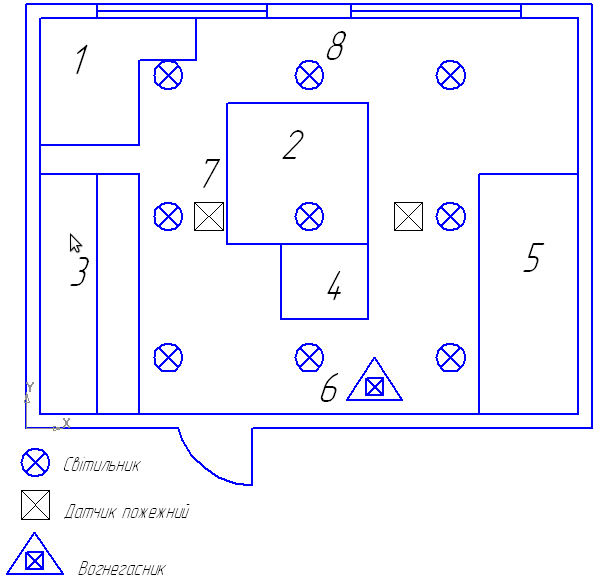
\includegraphics[scale=0.6]{lab_plan}
\caption{План робочого приміщення}\label{fig:lab_plan}
\end{figure}

\begin{enumerate}
 \item Робоче місце №1;
 \item Координатна платформа;
 \item Робоче місце №2;
 \item Стіл з ПК приєднаний до мережі та до вимірювальної апаратури;
 \item Шафа з допоміжним обладнанням та витратними матеріалами;
 \item Вогнегасник;
 \item Датчик пожежний;
 \item Світильник.
\end{enumerate}

В приміщенні розташовані два робочих місця. Перше обладнане ПК з рідкокристалічним дисплеєм, приєднане до локальної мережі. На столі додатково встановлені програматори, осцилограф, лабораторний блок живлення та мультиметр, телефон, принтер. Друге робоче місце обладнане паяльною станцією, контрольно-вимірною апаратурою, лабораторним блоком живлення, та додатковими розетками з мережею живлення 115В 400Гц. ПК, приєднаний до локальної мережі Ethernet. Над столом знаходиться полиця з радіоелементами. Всі прилади мають бути заземлені.

Трудова діяльність інженера програміста відбувається у певному виробничому середовищі, де діють такі шкідливі фактори: 
\begin{enumerate}
  \item Понижений рівень штучного освітлення 
  \item Мікроклімат
  \item Електричний струм
  \item Пожежонебезпека
  \item Шум

\end{enumerate}
% Освітлення
% Мікроклімат виробничих приміщень
% Шкідливі речовини в повітрі робочої зони
% 
% Шум, вібрація, ультразвук, інфразвук
% Виробничі випромінювання
% Небезпека ураження електричним струмом


Оптимальні умови мікроклімату встановлюються для постійних робочих місць. Показники температури повітря в робочій зоні по висоті та горизонталі протягом робочої зміни не повинні виходити за межі нормованих величин. Для інженера програміста відповідно до ДСН 3.3.6.042-99, для категорії робіт 1а, оптимальна температура повітря має становити в холодну пору $22-24^o$ С, відносна вологість 60-40\% швидкість руху повітря не більше 0.1 м/с.

Допустимі рівні звукового тиску у октавних смугах частот, еквівалентні рівні звуку на робочому місці регламентовані ДСН 3.3.6.037-99, для інженера показані в таблиці \ref{tb:noise}.
\begin{table}[H]
\small
\caption{Нормовані рівні звукового тиску та рівень шуму на робочому місці}
\centering
\begin{tabular}{|p{0.4in}|p{0.4in}|p{0.4in}|p{0.4in}|p{0.4in}|p{0.4in}|p{0.4in}|p{0.4in}|p{0.4in}|p{0.4in}|} \hline 
\multicolumn{9}{|p{4in}|}{Рівні звукового тиску (дБ) в  октавних смугах з серединами геометричними частотами, Гц} & Рівень звуку, дБА \\ \hline 
31.5 & 63 & 125 & 250 & 500 & 1000 & 2000 & 4000 & 8000 & 50 \\ \hline 
86 & 71 & 61 & 54 & 49 & 45 & 42 & 40 & 38 &  \\ \hline 
\end{tabular}
\label{tb:noise}
\end{table}
Методи вимірювання шуму, інфразвуку та ультразвуку регламентовано ДСН 3.3.6.037-99. Вплив шуму на людину, його вимірювання та оцінювання, для присутньої обчислюваної та офісної техніки здійснюється відповідно до ДСТУ ISO 7779:2005, а присутні кондиціонер за ДСТУ 3010-95. 

Якщо лабораторія знаходиться не далеко від аеродрому, необхідна додаткова звукоізоляція. У якості звукоізолюючих матеріалів, які застосовують у конструкціях перекриттів для зниження передачі структурного (ударного) звуку переважно використовують мати та плити із скляного та мінерального волокна, м'які плити з деревних стружок, картон, гуму, утеплений лінолеум.

Особу увагу необхідно приділити важливому з точки зору виробничої санітарії питанню освітлення на робочому місці. Основним документом, який регламентує норми освітленості є ДБН.В.2.5-28-2006 <<Природне і штучне освітлення>>. 

Освітлення на робочому місці повинно бути поєднаним (штучне та природне світло). 
Природне освітлення повинно бути боковим. При виконанні робот з категорії високої 
зорової точності коефіцієнт природної освітленості повинен відповідати нормативним 
рівням по ДБН.В.2.5-28-2006 (не нижче 1,5), при зоровій роботі середньої точності – не нижче 1.

Освітлення повинно бути достатнім, щоб очі без зайвого напруження могли розрізняти деталі, що розглядаються; стабільним – для цього напруга в електричній мережі не повинна коливатися більше ніж на 4 \%; рівномірно розподіленим по робочих поверхнях, щоб очам не доводилося потрапляти з дуже темного місця у світле і навпаки; таким, що не викликає сліпучої дії на око людини як самого джерела світла, так і від відбиваючих поверхонь, що знаходяться в полі зору робітника. 
Зменшення віддзеркалювання джерел світла досягається шляхом застосування світильників; 
таким, щоб не викликати різкі тіні на робочих місцях (цього можна досягти при правильному розташуванні світильників); 
безпечним – не призводити до вибуху, пожежі у виробничих приміщеннях.

Для створення сприятливих умов зорової роботи освітлення робочих приміщень задовольняються наступні умови:
\begin{enumerate}
 \item рівень освітленості робочих місць відповідає гігієнічним нормам для даного виду роботи;
 \item забезпечена рівномірність та часова стабільність рівня освітленості у приміщенні, відсутні різкі контрасти між освітленою робочою зоною та навколишнім простором;
 \item відсутні різкі та рухомі тіні;
 \item у полі зору предмета немає сліпучого блиску
 \item штучне світло за спектральним складом наближається до природного
\end{enumerate}

Розрахунок виробничого освітлення зроблено за методом використання 
світлового потоку. За цім методом світловий потік однієї лампи (у люменах) визначається за формулою:
\begin{equation}
\label{eq:fnop}
 F_n = \frac{E_{n}SkZ}{n \eta}
\end{equation}
\begin{ESKDexplanation}
\item де $E_n$ -- нормована освітленість для проектованих ділянок, цехів, лабораторій;
\item S – площа приміщення, у якому проектується виробниче освітлення, м2;
\item k – коефіцієнт запасу світлового потоку. Він приймається: для люмінесцентних ламп при малому виділенні пилу, диму, кіптяви - 1,5, при середньому і великому виділенні відповідно -1,8 й 2,0; для ламп накалювання при малому виділенні пилу, диму, кіптяви - 1,3, при середньому й великому, відповідно - 1,5 й 1,7;
\item Z – поправочний коефіцієнт, що відбиває відношення  , приймається при найвигіднішому розташуванні світильників, коли світловий потік використається для освітлення робочої зони найбільш раціонально, рівним 1,1-1,2; 
\item n – число ламп в приміщенні;
\item  $\eta$ – коефіцієнт використання світового потоку від світильника, що показує, яка частина світлового потоку лампи   досягає освітлюваної поверхні, у тому числі завдяки відбиттю світлового потоку від стін, стелі й робочої поверхні.
Коефіцієнт $\eta$, що залежить від показника геометричних розмірів приміщення   і коефіцієнтів відбиття стін  , стелі   і приміщення  , обчислений для різних типів світильників.	  
\end{ESKDexplanation}

Показник  приміщення:
\begin{equation}
\label{eq:iop}
 i = \frac{a \times b}{H(a+b)}= \frac{5 \times 6}{1,925(6+5)}
\end{equation}
\begin{ESKDexplanation}
  \item де a та b – довжина й ширина освітлюваного приміщення, м;  
  \item H – висота підвісу світильників над робочою поверхнею, м.
\end{ESKDexplanation}

Висота підвісу знаходить з наступної формули:
\begin{equation}
\label{eq:hop}
 H =h_{b} - N - h_{c} 
\end{equation}   
\begin{ESKDexplanation}
\item де $h_{b}$ – висота приміщення, м;
\item $h_{с}$ – висота світильника, м;
\item N – висота робочої поверхні, м.
\end{ESKDexplanation}
Приміщення лабораторії має наступні геометричні формули: довжина робочого кабінету складає 6 м;
ширина - 5 м; висота - 3 м. Визначимо висоту підвісу світильників, підставив вихідні значення в формулу \ref{eq:hop}:
\begin{equation}
 H =   3,0 - 0,275 - 0,8 = 1,925(m).
\end{equation}
тоді індекс приміщення:
\begin{equation*}
 i =  \frac{5 \times 6}{1,925(6+5)}= 1.41676
\end{equation*}            

Далі визначимо значення показника приміщення, підставляючи в формулу значення :       
По показнику приміщення та коефіцієнтам світлового потоку від підлоги – 10\% (0,1), від стін – 30\% (0,3) та від стелі – 80\% (0,8)
визначаємо для світлодіодної лампи ML-T8-13W/0.6-SMD значення коефіцієнта використання світлового потоку ($\eta$). $\eta$ = 0,69; коефіцієнт запасу світлового потоку k = 1,25; поправочний коефіцієнт Z = 1,2. 

Норма (мінімум) освітленості при проведенні середньо точних робіт складає 400 лк.Світловий потік лампи ML-T8-13W/0.6-SMD складає 1950 лм. З формули \ref{eq:fnop} виразимо число ламп в приміщенні та підставляючи відомі значення в вираз одержимо
 
\begin{equation}
 n = \frac{400 \times 30 \times 1.25 \times 1.2 }{1750 \times 0.69} = 18
\end{equation}

Округляючи значення до більшої цілої цифри, отримуємо, що вимагається 18 ламп. Якщо в світильник 2 лампи то нам необхідно 9 світильників.

 Приміщення, призначені для роботи ПК, повинні мати природне освітлення. Орієнтація вікон повинна бути на північ або на північний схід, вікна повинні мати жалюзі, які можна регулювати, або штори.

% Не дозволяється розміщувати кабінети обчислювальної техніки у підвальних приміщеннях будинку. Кабінети, обладнанні комп’ютерною технікою, повинні розміщуватись в окремих приміщеннях з природнім освітленням і організованим обміном повітря. Площа на одного працюючого за ПК повинна складати неменше $6 m^2$, об’єм  - не менше $20 m^3$. Стіни , стеля і підлога та обладнання кабінетів комп’ютерної техніки повинні мати покриття із матеріалів з матовою структурою з коефіцієнтом відбиття: стін --- 40--50\%, стелі --- 70--80\%, підлоги --- 20--30\%, предметів обладнання --- 40--50\% (робочого столу  --- 40--50\%, корпуса дисплею та  клавіатури --- 30--50\%, шаф та стелажів --- 40--60\%).
\subsection{Забезпечення пожежної безпеки в розроблювальному проекті}
Пожежна безпека забезпечена у відповідності з НАПБ А.01.001-2004 <<Правила пожежної безпеки в Україні>>, який є обов'язковим для виконання всіма підприємствами не залежно від форми власності. Правила встановлюють загальні вимоги з пожежної безпеки. Забезпечуючи пожежну безпеку, слід також керуватись ПУЕ та НПАОП 40.1-1.32-01 <<Правила побудови електроустановок.Електрообладнання спеціальних установок>> та інших нормативних документів, що стосуються штучного освітлення і електротехнічних пристроїв, а також вимог нормативно-технічної експлуатаційної документації заводу-виробника.

Робоче приміщення лабораторії за класифікацією пожежонебезпечності має відноситься до категорії Д.

Забезпечення пожежної безпеки в лабораторії досягається за рахунок застосування мір пожежної профілактики 
й активного пожежного захисту, тобто комплексу мір попередження виникнення пожеж або зменшення їх наслідків. Причинами виникнення пожежі електроустаткування можуть бути:
\begin{enumerate}
 \item перевантаження проводів;
 \item неякісне виконання з'єднань електропроводки;
 \item перевантаження різних електричних пристроїв;
 \item коротке замикання
 \item контакт горючих речовин з нагрівальними пристроями.
\end{enumerate}

%Відповідно до ДНАОП 0.00-1.31-99, під час проектування систем електропостачання, монтажу 
%основного електрообладнання та електричного освітлення приміщень для ЕОМ дотримано вимог 
%Правил влаштування електроустановок (ПВЕ), ГОСТ 12.1.006-84, ГОСТ 12.1.019-79, ГОСТ 12.1.030-81, 
%ГОСТ 12.1.045-84, ПТЕ, ПБЕ, ВСН 59-88,  СН 357-77, 



%Комплекс виробничих приміщень має два евакуаційних виходи.Приміщення де зберігається інформація відокремлене і  обладнане шафами з негорючих матеріалів (метал).
%Для запобігання загоряння від світильників у приміщенні, використовують лампи з температурою нагрівання зовнішніх стекол закритих плафонах. Загальні вимоги пожежної та вибухової безпеки наведені відповідно в ГОСТ12.1.004-91 та ГОСТ 12.1.010-76.

Джерела електричної енергії (розподільчі пристрої, трансформатори) розташовувані у відокремлених приміщеннях.

Освітлювальну електричну мережу виконано згідно вимог ПЕУ – правилам устрою електроустановок для пожежонебезпечних зон.
Прокладання кабелю через перекриття, стіни, фальшпідлогу здійснено в стальних трубах з наповнювачем з негорючих матеріалів. Аварійні мережі освітлення, дистанційного та автоматичного пуску протипожежних систем та сигналізації 
прокладено окремо від силових та інших електричних комунікацій, а при сумісному прокладанні їх 
розділено перегородками з негорючих матеріалів (метал, гетинакс).


Повітропроводи виконані з негорючих матеріалів. Система вентиляції обладнана пристроєм, що 
забезпечує автоматичне її відключення, а також перекриття повітропроводів лабораторії 
автоматичними заслінками в разі виникнення пожежі. Кабельні вертикальні шахти розділені 
по поверхах діафрагмами з негорючих матеріалів.

Ефективність застосування вогнегасника, у першу чергу пов’язана з правильним вибором його типу залежно від класу пожежі, яку не необхідно погасити. Основні вимоги до оснащення об’єктів вогнегасниками регламентуються НАПБ Б.03.001-2004 Типові норми належності вогнегасників. При експлуатації вогнегасників слід керуватись НАПБ Б.01.008-2004 Правила експлуатації вогнегасників.

Для гасіння та локалізації пожежі до прибуття пожежних підрозділів використовуються ручні вогнегасники.  У приміщенні необхідний 1  вуглекислотний вогнегасник типу ВВ (ВВ-2, ВВ-5, ВВ-8). Застосування вуглекислотних вогнегасників зумовлено тим, що вони можуть використовуватися для гасіння дорогого обладнання, яке знаходиться під напругою до 1000 В. 

Для виявлення пожежі використовують пожежно-охоронну сигналізацію, у відповідності до ДСТУ EN54-2:2003. Пожежні сповіщувачі використовуються для формування командного імпульсу автоматичного пуску системи автоматичного пожежегасіння. Кількість теплових пожежних сповіщувачів визначається за таблицею і для приміщення розмірами 6 х 5 х 3 м становить 2. 
Температура спрацювання сповіщувачів встановлюється не менше ніж на $20^o$С вище 
максимальної припустимої температури в приміщенні.

Для виявлення пожежі, замість старик точкових пристроїв пропонується встановити датчики Honeywell Notifier SFAPT-453(A)
(Acclimate PlusTM Multi-Sensor Low-Profile Smoke Intelligent Detector). Датчик використовує аналізатор диму та комбінацію фотоелектричних та температурних сенсорів з вмонтованим для підвищення імунітету до фальшивого спрацювання. Пристрій обладнаний мікропроцесором для обробки інформації, в результаті він налаштовує чутливість автоматично не залежно від оператора контрольної панелі та проводить самотестування. Іншою перевагою, даного типу датчика є, його безпосередня зв'язаність з системою кондиціювання та вентиляції. В разі пожежі вимикається та блокується кондиціонер,
і закриваються заслонки вентиляційної системи.

Дані з сенсорів подаються на загальну панель керування пожежно-охоронної системи сигналізації, а далі на пост чергового пожежної частини. Оператор або панель керування автоматично приймають рішення, щодо вимкення постачання електроенергії
до приміщення лабораторії

Евакуація здійснюється відповідно до НАПБ А.01.003-2009 "Правила улаштування та експлуатації систем оповіщення про пожежу та управління евакуацією людей в будинках та спорудах". Комплекс виробничих приміщень має два евакуаційних виходи. Двері на шляхах евакуації мають відчинятися у напрямку виходу зі споруди, ширина шляхів -- не менше 1м, а ширина дверей -- 0.8м.

\subsection{Електробезпека}

Відповідно до НАОП 0.00-1.28-10 Правила охорони праці під час експлуатації електронно-обчислювальних машин, ЕОМ з ВДТ і ПП, інше устаткування (апарати управління, контрольно-вимірювальні прилади, світильники), електропроводи та кабелі за виконанням і ступенем захисту мають відповідати класу зони за НПАОП 40.1-1.01-97, мати апаратуру захисту від струму короткого замикання та інших аварійних режимів.

Під час монтажу та експлуатації ліній електромережі необхідно повністю унеможливити виникнення електричного джерела загоряння внаслідок короткого замикання та перевантаження проводів, обмежувати застосування проводів з легкозаймистою ізоляцією і, за можливості, застосовувати негорючу ізоляцію.

Під час ремонту ліній електромережі шляхом зварювання, паяння та з використанням відкритого вогню необхідно дотримуватися НАПБ А.01.001-2004.

Лінія електромережі для живлення ЕОМ з ВДТ і ПП виконується як окрема групова трипровідна мережа шляхом прокладання фазового, нульового робочого та нульового захисного провідників. Нульовий захисний провідник використовується для заземлення (занулення) електроприймачів.
Не допускається використовувати нульовий робочий провідник як нульовий захисний провідник.

Нульовий захисний провідник прокладається від стійки групового розподільного щита, розподільного пункту до розеток електроживлення.

Не допускається підключати на щиті до одного контактного затискача нульовий робочий та нульовий захисний провідники.

Площа перерізу нульового робочого та нульового захисного провідника в груповій трипровідній мережі має бути не менше площі перерізу фазового провідника. Усі провідники мають відповідати номінальним параметрам мережі та навантаження, умовам навколишнього середовища, умовам розподілу провідників, температурному режиму та типам апаратури захисту, вимогам НПАОП 40.1-1.01-97.

У приміщенні, де одночасно експлуатуються понад п'ять ЕОМ з ВДТ і ПП, на помітному та доступному місці встановлюється аварійний резервний вимикач, який може повністю вимкнути електричне живлення приміщення, крім освітлення.

ЕОМ з ВДТ і ПП повинні підключатися до електромережі тільки за допомогою справних штепсельних з'єднань і електророзеток заводського виготовлення.
У штепсельних з'єднаннях та електророзетках, крім контактів фазового та нульового робочого провідників, мають бути спеціальні контакти для підключення нульового захисного провідника. Їхня конструкція має бути такою, щоб приєднання нульового захисного провідника відбувалося раніше, ніж приєднання фазового та нульового робочого провідників. Порядок роз'єднання при відключенні має бути зворотним.

Не допускається підключати ЕОМ з ВДТ і ПП до звичайної двопровідної електромережі, в тому числі - з використанням перехідних пристроїв.

Електромережі штепсельних з'єднань та електророзеток для живлення ЕОМ з ВДТ і ПП потрібно виконувати за магістральною схемою, по 3-6 з'єднань або електророзеток в одному колі.

Штепсельні з'єднання та електророзетки для напруги 12 В та 42 В за своєю конструкцією мають відрізнятися від штепсельних з'єднань для напруги 127 В та 220 В.
Штепсельні з'єднання та електророзетки, розраховані на напругу 12 В та 42 В, мають візуально (за кольором) відрізнятися від кольору штепсельних з'єднань, розрахованих на напругу 127 В та 220 В.

Індивідуальні та групові штепсельні з'єднання та електророзетки необхідно монтувати на негорючих або важкогорючих пластинах з урахуванням вимог НПАОП 40.1-1.01-97 та НАПБ А.01.001-2004.

Електромережу штепсельних розеток для живлення ЕОМ з ВДТ і ПП при розташуванні їх уздовж стін приміщення прокладають по підлозі поруч зі стінами приміщення, як правило, в металевих трубах і гнучких металевих рукавах, а також у пластикових коробах і пластмасових рукавах з відводами відповідно до затвердженого плану розміщення обладнання та технічних характеристик обладнання.
При розміщенні в приміщенні до п'яти ЕОМ з ВДТ і ПП допускається прокладання трипровідникового захищеного проводу або кабелю в оболонці з негорючого чи важкогорючого матеріалу по периметру приміщення без металевих труб та гнучких металевих рукавів.

При організації робочих місць операторів електромережу штепсельних розеток для живлення ЕОМ з ВДТ і ПП у центрі приміщення прокладають у каналах або під знімною підлогою в металевих трубах або гнучких металевих рукавах. При цьому не допускається застосовувати провід і кабель в ізоляції з вулканізованої гуми та інші матеріали, які містять сірку.


\subsection{Висновок}
В роботі проаналізовано основні небезпечні чинники, можна відзначити, що при дотриманні правил безпеки і виробничої санітарії обладнання навігаційної системи не є пожежонебезпечним. Запропоновані світлодіодні лампи є не тільки економічними але й створюють оптимальні умови для зорової роботи інженера програміста, а порівняно не висока температура нагрівання підвищує рівень пожежної безпеки.


% 
% 
% При реалізації проекту на працівників можуть впливати шкідливі і небезпечні виробничі чинники: підвищений 
% рівень рентгенівських випромінювань, недостатнє  освітлення робочої зони, підвищене значення напруги електричного 
% струму, який може проходити крізь людину при коротких замиканнях електричної мережі, підвищений рівень шуму внаслідок
% роботи оргтехніки.
% 
% Електронно-променеві трубки, працюючи при напругах понад 6 кВ є джерелами "м'якого" рентгенівського випромінювання. 
% При напругах понад  10 кВ рентгенівське випромінювання виходить за межі скляного балону і розсіюється в 
% навколишньому просторі виробничого приміщення.
% 
% В силу тісного взаємозв'язку зору людини з роботою мозку освітлення виявляє істотний вплив на центральну нервову 
% систему, керуючу всією життєдіяльністю людини. Раціональне освітлення сприяє підвищенню продуктивності і безпеки 
% праці і збереженню здоров’я працюючих.
% 
% Недостатнє освітлення робочих місць може виникати з таких причин: невірне розташування сусідніх будівель, які 
% можуть створювати затемнення робочої зони; забруднення та недостатня кількість або непрацездатність деяких чи 
% всіх освітлювальних приладів; невірно підібрані чи замінені лампи в світильниках та інші.
% 
% При технічній експлуатації електричного обладнання  можуть виникати електротравми з таких причин: безпосереднє 
% доторкання чи доторкання інструментом до струмопровідних частин електроустановок під напругою, внаслідок невірних 
% дій персоналу, недотримання правил техніки безпеки або внаслідок помилок при монтажі схем і елементів; ураження 
% шаговою напругою при дотику до стін, підлоги, які опинились під напругою по причині погіршення ізоляції чи падінні дротів.  
% 
% \subsection{Технічні заходи щодо ліквідації і зниження дії небезпечних
%  і шкідливих виробничих факторів}
% 
% Приміщення, призначені для роботи ПК, повинні мати природне освітлення. Орієнтація вікон повинна бути на північ або на північний схід, вікна повинні мати жалюзі, які можна регулювати, або штори.
% Не дозволяється розміщувати кабінети обчислювальної техніки у підвальних приміщеннях будинку. Кабінети, обладнанні комп’ютерною технікою, повинні розміщуватись в окремих приміщеннях з природнім освітленням і організованим обміном повітря. Площа на одного працюючого за ПК повинна складати неменше $6 m^2$, об’єм  - не менше $20 m^3$. Стіни , стеля і підлога та обладнання кабінетів комп’ютерної техніки повинні мати покриття із матеріалів з матовою структурою з коефіцієнтом відбиття: стін --- 40--50\%, стелі --- 70--80\%, підлоги --- 20--30\%, предметів обладнання --- 40--50\% (робочого столу  --- 40--50\%, корпуса дисплею та  клавіатури --- 30--50\%, шаф та стелажів --- 40--60\%). Поверхня підлоги повинна  мати антистатичне покриття та бути зручною для вологого прибирання. Забороняється використовувати для оздоблення інтер’єру  комп’ютерних приміщень полімерні матеріали (дерев’яно-стружкові плити, шпалери,що придатні для миття, плівкові та рулонні синтетичні матеріали, шаровий пластик та ін.), що виділяють у повітря шкідливі хімічні речовини, які перевищують гранично допустимі концентрації.
% 
% Вміст шкідливих хімічних речовин в повітрі з комп’ютерною технікою не повинен перевищувати середньодобової концентрації, що наводяться в <<Переліку гранично допустимих концентрацій забруднюючих речовин в атмосферному повітрі населених пунктів> \No 3086-84 від 27.08.84 р. та доповненнях до нього, які затвердженні Міністерствам охорони здоров’я>>.
% Приміщення з ПК повинні мати природне та штучне освітлення. Природне освітлення повинно відповідати вимогам ДБНВ 2.2-3-97  <<Будинки та споруди навчальних закладів>>. Штучне освітлення в приміщеннях з ПК повинно здійснюватись системою загального освітлення. Як джерела світла при штучному освітленні повинні застосовуватись люмінесцентні лампи. Штучне освітлення повинно забезпечувати на робочих місцях в кабінетах з ПК освітленість не нижчу, а на екранах дисплеїв – не вище приведених в таб. \ref{tab:labour protection}
% 
% \begin{table}
% \centering
% \begin{tabular}[c]{|p{5cm}|c|c|c|c|}
% \hline
% \bfseries Характеристика & \bfseries Робоча & \bfseries Площина & \bfseries Освітленість& \bfseries Примітка \\ 
% \bfseries роботи         & \bfseries поверхня & &\bfseries , лк  & \\
% 
% \hline
% Робота переважно з екранами дисплеїв ПК (50\% робочого часу)
% & Екран & В & 200 & не вище \\ 
% & Клавіатура & Г & 400 & не нижче \\ 
% & Стіл & Г & 400 & не нижче \\ 
% 
% \hline
% Робота переважно з документами (з екранами дисплеїв ПК менше 50\% робочого часу)
% & Екран & В & 200 & не вище \\ 
% & Клавіатура & Г & 400 & не нижче \\ 
% & Стіл & Г & 500 & не нижче \\ 
% & Стенд & В & 500 & не нижче \\ 
% 
% \hline
% Проходи основні & Підлога & Г & 100 & \\
% \hline
% \end{tabular}
% \caption{норми освітленості в кабінетах з ПК}
% \label{tab:labour protection}
% \end{table} 
% 
% Загальне освітлення повинно бути виконано у вигляді суцільних або переривчатих  ліній світильників. Для загального 
% освітлення припустимо застосування світильників наступних класів світлорозподілу П (прямого світла), В 
% (переважно  відбитого с вітла).  Застосування   світильників   без   розсіюваів   та екрануючих гратів заборонено. 
% Яскравість світильників загального освітлення в зоні кутів випромінювання від 50$^{\circ}$ до 90$^{\circ}$ з вертикаллю в поздовжній та поперечних площинах повинна складати не быльше 200 кд/кв.м, захисний кут світильників повинен бути не менше 40$^{\circ}$. Коефіціент запаса (КЗ) для освітлювальних установок загального освітлення приймається рівним 1,4. Співвідношення яскравості між робочим екраном і близьким оточенням (стіл, книжки та ін.) не повинно перевищувати 5:1, між поверхнями робочого екрану і оточенням (стіл, обладнання) – 10:1. Величина коефіціенту пульсації освітлення не повиннв перевищувати 5\%. Необхідно передбачити обмеження прямої блискості від джерел природного та штучного освітлення. Яскравість великих поверхонь (вікна, світильники), що знаходяться у полі зору, не повинна перевищувати 200 кд/кв. м. Показник освітленості для джерел штучного освітлення у кабінетах з ВДТ не повинен бути більшим 20.
% 
% Мірою захисту від прямої блискості має бути зниження яскравості видимої частини джерел світла шляхом застосування розсіювачів, відбивачів та інших світлозахисних пристроїв, а також правильне розміщення робочих місць відносно джерел світла.
% 
% У робочій зоні виробничих приміщень ДЕСТ 12.1.005-88 ССБТ «Загальні санітарно-гігієнічні вимоги до повітря робочої зони» установлює норми температури, відносній вологості і швидкості руху повітря в теплий, холодний і перехідний періоди року, виходячи з категорії роботи по складності, призначенню приміщень, надлишкам тепла. Оптимальні параметри повітряного середовища забезпечуються застосуванням опалення, вентиляції і кондиціонування повітря відповідно до вимог БНіП 2.04.05-92 <<Опалення, вентиляція і кондиціонування повітря>>.
% 
% Забезпечення нормальних метеорологічних умов у робочій зоні виробничих приміщень домагаються 
% постійним контролем за ними і проведенням спеціальних заходів. Контроль за станом повітряного 
% середовища повинний виконуватися  з використанням термометрів і термографів (термографи 
% автоматично записують поточну температуру), психрометрів і гігрометрів (для виміру вологості), 
% актинометрів  (для  виміру  інтенсивності  теплових  випромінювань.  У  холодні  і  теплі 
% періоди року температура повітря, швидкість його руху і відносна вологість повітря повинні 
% відповідно складати: 18--20 $^{\circ}$С; 0,1--0,2 м/с; 60--40\%; температура повітря може 
% коливатися  від 16 до 23 $^{\circ}$С при збереженні інших параметрів мікроклімату  в зазначених вище межах. 
% У теплі періоди року температура повітря, його рухливість і відносна вологість повинні 
% відповідно складати: 21--23 $^{\circ}$С; 0,2--0,3 м/с; 60--40\%; температура повітря може 
% коливатися від 18 до 25 $^{\circ}$С при збереженні інших параметрів мікроклімату в зазначених вище межах.
% 
% Заходи, що забезпечують нормальні метеорологічні умови : 
% \begin{enumerate}
%  \item ізоляція джерел надлишкового тепла, їхнє екранування і раціональне розташування, що зменшує схрещування променистих потоків тепла на робочому місці;
%  \item пристрій приточно-витяжної вентиляції, що забезпечує видалення надлишкового тепла і вологи з приміщення, багаторазову зміну повітря й охолодження  організму чи  нагрівання у випадку кондиціонування повітря;
%  \item застосування повітряного душу при трудових процесах, коли інтенсивність теплового випромінювання велика або тепловіддача в навколишнє середовище утруднена.
% \end{enumerate}
% 
% В відповідності з вимогами, гранично допустимі рівні напруги дотику і 
% струмів при експлуатації і ремонті обладнання забезпечуються: застосуванням малих напруг; ізоляцією струмопровідних мереж; 
% обґрунтуванням і оптимальним вибором елементної бази, що виключає передумови 
% поразки електричним струмом; правильної компонування, монтажем приладів і елементів; 
% дотриманням умов безпеки при постанові і заміні приладів і ін.
% 
% Одним із засобів, що забезпечують безпеку людини, що працює з ЕОМ, є --- захисне заземлення. 
% Захисним є заземлення, що полягає в надійному з'єднанні  корпуса чи  металевих неструмоведучих 
% частин електроустановки з землею. Принцип дії захисного заземлення --- зниження до безпечних значень 
% напруги дотику і кроку, обумовлених замиканням на корпус. Напруга, під якою опиняється людина під час  
% дотику до корпуса електроустановки – Uч, rзаз - опір заземлення. Для зниження напруги необхідно зменшити 
% опір заземлення. Таким чином, з'єднуючи корпус електроустановки з землею, можна знизити напругу, 
% що прикладається до тіла людини, до такого значення, при якому струм, що протікає через нього, не 
% представляє  смертельної небезпеки .
% 
% Приклад: Розрахувати загальне освітлення ділянки дефектації вузлів авіаційних двигунів, де норма освітленості при застосуванні люмінесцентних ламп (розряд ) – 400 лк. Розміри приміщення: А = 40 м; В = 20 м; H = 3,0 м. Передбачається використовувати світильники типу ШОД з лампами ЛД, висота підвісу над робочою поверхнею hр = 2,5 м, коефіцієнт запасу приймаємо рівним 1,5 аналогічно приміщенням з малим виділенням пилу, диму і кіптяви.
% Визначимо показник приміщення:
% 
% Задавшись значеннями коефіцієнтів відбиття стелі $p = 0,7$; стін $\rho_z = 0,1$ і освітлюваної поверхні $\rho_p = 0,1$; за спеціальними таблицями знаходимо коефіцієнт використання світлового потоку світильника $\eta = 0,59$. Поправочний коефіцієнт Z приймаємо рівним 1,1.
% 
% Подальший розрахунок може зводитися до визначення необхідного світлового потоку однієї лампи, якщо відома кількість світильників і ламп у них, або до визначення кількості світильників і ламп, якщо відомий тип і потужність ламп.
% 
% Якщо в нашому прикладі передбачається використовувати світильники ШОД з лампами ЛД 2x80, $F = 13200$ лм, то кількість ламп знайдемо з виразу
% 
% Отже, світильники слід розташовувати рівномірно в трьох рядах по одинадцять штук.
% 
% Даний приклад показує нам як необхідно розраховувати виробниче освітлення. Маючи усі данні ми можемо розрахувати виробниче освітлення в необхідному нам приміщенні.
% 
% \subsection{Забезпечення пожежної і вибухової безпеки спроектованого 
%  об'єкта}
% 
% Загальні вимоги по забезпеченню пожежної та вибухової безпеки об’єктів виробничого призначення визначені відповідно у ДЕСТ 12.1.004-91 та ДЕСТ 12.1.010-76.
% 
% Пожежна небезпека може бути обумовлена утворенням електричної дуги, іскор, перегріву струмопровідних елементів.
% Вибухова небезпека відсутня згідно ДЕСТ 12.1.010-76, тому що відсутні джерела їх виникнення.
% 
% Заходи по забезпеченню пожежної безпеки :
% 
% \begin{enumerate}
%  \item лабораторії розміщаються в будівлях не нижче П ступіні вогнетривкості;
%  \item комплекс виробничих приміщень лабораторій має не менш двох самостійних евакуаційних виходів;
%  \item для акустичного оздоблення стін використані негорючі матеріали, які під впливом вогню або високої температури не загоряються, не тліють та не обвуглюються: до негорючих матеріалів відносять усі природні або штучні неорганічні матеріали, а також метали, які використовуються в будівництві.
%  \item джерела електричної енергії (розподільчі пристрої, трансформатори) знаходяться у відокремлених приміщеннях;
%  \item прокладка кабелів через перекриття, стіни здійснюється в сталевих трубах з ущільненням із негорючих матеріалів;
%  \item система вентиляції обладнана пристроєм, який забезпечує її автоматичне вимкнення у випадку пожежі.
% \end{enumerate}
% 
% При виникненні пожежі потрібно вивести людей і матеріальні цінності з небезпечної зони, викликати пожежну охорону, вжити міри по локалізації пожежі, по можливості, вжити міри по гасінню пожежі.
% 
% В приміщеннях є установки гасіння пожеж газовими вогнегасники засобами, в яких вогнегасною речовиною є вуглекислота. Можна також застосовувати для гасіння повітряно-механічну піну, завчасно знеструмив установки, тому що піна є електропроводною. 
% 
% Для гасіння пожеж в лабораторії застосовують переносні вуглекислотні вогнегасники, які установляються з розрахунку: 1 вогнегасник на 40-50 м2 полу.
% 
% Для виявлення пожежі в приміщеннях установлені датчики Honeywell Notifier FAPT-851(A)
% (Acclimate PlusTM Multi-Sensor Low-Profile Intelligent Detector). Датчик 
% використовує комбінацію фотоелектричних та температурних сенсорів для
% підвищення імунітету до фальшивого спрацювання. Датчик обладнаний мікропроцесором
% для обробки інформації, в результаті він налаштовує чутливість автоматично
% не залежно від оператора контрольної панелі та проводить самотестування.
% 
% Дані з сенсорів подаються на загальну панель керування пожежно-охоронної системи
% сигналізації та на
% 
% 
% 
% 
% \subsection{Інструкція з охорони праці під час виконання робіт зі 
%  спроектованим об'єктом}
% Інструкція складена відповідно до вимог ДНАОП 0.00-4.15-98  <<Положення про розробку інструкцій з охорони праці>>.
% 
% До роботи з проектованим об'єктом допускаються обличчя інженерно-технічного складу, що вивчили проектований пристрій, інструкцію з технічної експлуатації, дійсну інструкцію і що склали залік по техніці безпеки і пожежної безпеки.
% \begin{enumerate}
%  \item Упорядкувати робоче місце. 
%  \item Перевірити  справність роз’ємів кабелів електроживлення і блоків пристроїв, відсутність зламів і ушкоджень ізоляції живильних проводів, відсутність відкритих струмоведучих частин у пристроях ПК;
%  \item Відрегулювати сидіння робочого стільця (крісла) на оптимально зручну висоту      (кут нахилу спинки стільця повинний змінюватися в межах 90-11-град. до площини сидіння).
%  \item Розташувати крісло і дисплей так, щоб кут зору на екрані складав 15 град., а відстань до екрана 400-800 мм;
%  \item Вжити заходів, щоб при нормальній освітленості робочого місця пряме світло не падало на екрани моніторів.
%  \item Перед включенням штепсельної вилки кабелю електроживлення в розетку 220 В переконайтеся в тому, що усі вимикачі мережі на всіх пристроях ПК знаходяться в положенні «заземлені» (занулені).
%  \item Після підключення пристроїв ПКдо електромережі установіть яскравість і фокус зображення ВДТ ручками регулювання відповідно до особливості свого зору.
%  \item Не залишати свого робочого місця без повідомлення керівника робіт.
%  \item Не залишати працюючий ПКі його пристрої без спостереження.
%  \item Підключати і відключати роз’єми кабелів пристроїв ПК тільки при відключеній напрузі електричної мережі.
%  \item Подавати напругу на пристрої й окремі блоки ПК тільки після ретельної перевірки надійності кріплення провідників заземлення, справності кабелів і роз’ємів мережі електроживлення.
%  \item Для операторів ПК повинні бути додатково введені дві-три регламентованих перерви тривалістю 10 хвилин кожна, дві перерви при 8-мигодинному робочому дні, три перерви при 12-тигодинному робочому дні. 
%  \item Кількість оброблюваних символів (чи знаків ВДТ) не повинна перевищувати 30 тис. за 4 години роботи.
%  \item Установити в положення «виключено» усі тумблера (вимикачі) пристроїв, з якими ви працювали, а також перемикачі (рубильники) на електрощитах.
%  \item Відключити штепсельні вилки від розеток електроживлення.
%  \item Про всі несправності, виявлені під час роботи і про вжиті заходи з їхнього усунення, доповісти керівнику з відповідним записом у журналі обліку робіт.
%  \item Виключити загальний вимикач електроживлення всіх робочих місць.
%  \item Виключити світло на робочому місці й у приміщенні.
%  \item В аварійних ситуаціях:
%   \subitem Негайно припиніть роботу.
%   \subitem Залиште небезпечну зону і вживіть заходів з попередження подальшого розвитку аварії.
%   \subitem Повідомте про те, що трапилося, свого керівника, чи керівника ділянки, на якій відбулася аварія. 
%   \subitem При нещасних випадках забезпечте  долікарську допомогу потерпілому.
% \end{enumerate}
% 
% За порушення чи невиконання цих вимог винні несуть відповідальність відповідно до чинного законодавства.
\end{document}
